\chapter{Metodologie usate e raffinamenti successivi}

\section{Metodologia Agile}

L'intero ciclo di vita del software è stato gestito adottando una metodologia \emph{Agile}.

I metodi Agile sono tali da coinvolgere il più possibile il committente, dando quindi vita a un processo di tipo adattativo: cioè che si adatta alle esigenze del cliente, che possono cambiare durante lo sviluppo.
L'Agile è un processo costituito da finestre di tempo limitate (2-4 settimane) chiamate iterazioni, le quali sono a loro volta scomposte nelle fasi di progettazione, di sviluppo e di test.

\begin{figure}[htbp]
\centering
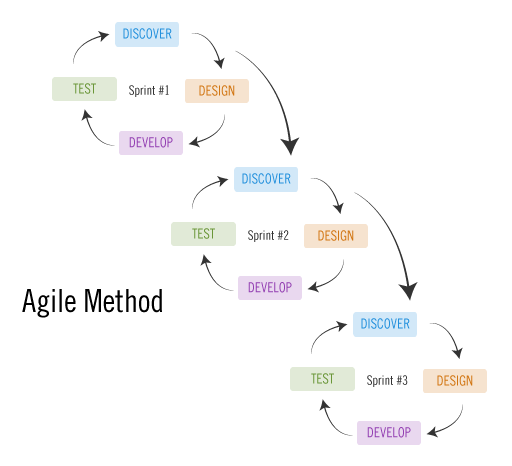
\includegraphics[scale=0.6]{immagini/agile.png}
\caption{Iterazioni e fasi della metodologia Agile}
\end{figure}

Il progetto è quindi suddiviso in singoli componenti indipendenti dalle funzionalità così da poterne analizzare e valutare i costi e i tempi. Ogni iterazione conterrà quindi tutto ciò che è indispensabile per rilasciare un piccolo incremento nelle funzionalità del software e sono tali da essere soggette a modifiche al fine di migliorare l'architettura finale del software.
% Anche se in un'iterazione non si hanno sufficienti funzionalità per ottenere un componente completo, esso deve esser rilasciato e nelle iterazioni successive dovrà avvicinarsi alle richieste del cliente.
% 
% Anche se il risultato di ogni singola
% iterazione non ha sufficienti funzionalità da essere considerato completo,
% deve essere rilasciato e nel susseguirsi delle iterazioni, deve avvicinarsi
% sempre di più alle richieste del cliente. Alla fine di ogni iterazione il team
% dovrà rivalutare le priorità del progetto.
% 
% Ogni iterazione è progetto a sé
% stante e deve contenere tutto ciò che è necessario per rilasciare un piccolo
% incremento nelle funzionalità del software: pianificazione (user stories),
% design, implementazione, test. An
% 
% Sulla scorta di queste considerazioni, nelle metodologie agili i vincoli principali dei progetti
% diventano i tempi, i costi e la possibilità di favorire la gestione del cambiamento dei requisiti.
% Naturalmente, per poter operare in tal modo, è richiesta la suddivisione in singoli componenti
% indipendenti delle funzionalità, al fine di poterne valutare i tempi, i costi e la possibilità di
% completarli procedendo per piccoli incrementi progressivi. In tal modo, viene agevolata anche la
% suddivisione dei compiti e delle responsabilità ai componenti del team di sviluppo.
% In definitiva, i Metodi Agili [21] sono un insieme di tecniche di sviluppo software che si
% focalizzano sullo sviluppo ed il rilascio incrementale (ed in tempi brevi) di porzioni del sistema, che
% siano usabili.
% 
% 
% 
% A differenza delle metodologie "pesanti", quelle agili sono caratterizzate da un processo
% iterativo scomposto in fase di progettazione, di sviluppo e test96 di breve durata.
% Tipicamente, i Metodi Agili si basano su di una disciplina rigorosa che dà vita ad un processo
% ben definito; si noti, però, che quest'ultimo è di tipo adattativo: si adatta, cioè, alle esigenze del
% committente, che possono mutare durante lo sviluppo. Quest'ultimo di focalizza su gruppi di
% funzionalità ed è guidato dalla necessità di rilasciare prodotti di progetto usabili.
% Dunque, gli artefatti possono considerarsi "leggeri", cioè manca la "pesante" documentazione.
% Il lavoro di progettazione, anzichè essere concentrato nella sola parte iniziale, è continuo e
% distribuito lungo tutte le fasi del processo. Pertanto, anche le parti già realizzate sono soggette a
% modifiche, al fine di migliorare l'architettura del software.
% 
% 
% Da ultima troviamo le metodologie agili. Questo particolare metodo di
% sviluppo software, a differenza dei precedenti, coinvolge quanto più
% possibile il committente, ottenendo in tal modo un elevata reattività alle
% sue richieste.
% La gran parte dei metodi agili tentano di ridurre il rischio di fallimento
% sviluppando il software in finestre di tempo limitate chiamate iterazioni
% che in genere durano qualche settimana. Ogni iterazione è progetto a sé
% stante e deve contenere tutto ciò che è necessario per rilasciare un piccolo
% incremento nelle funzionalità del software: pianificazione (user stories),
% design, implementazione, test. Anche se il risultato di ogni singola
% iterazione non ha sufficienti funzionalità da essere considerato completo,
% deve essere rilasciato e nel susseguirsi delle iterazioni, deve avvicinarsi
% sempre di più alle richieste del cliente. Alla fine di ogni iterazione il team
% dovrà rivalutare le priorità del progetto.
% 
% Un'importante constatazione che ha spinto verso questo approccio riguarda la natura mutevole
% nel tempo dei requisiti di un progetto. Pertanto, nell'ottica della pianificazione delle attività, i
% requisiti iniziali potrebbero risultare un punto di partenza inadeguato.
% L'adozione di un approccio è strettamente vincolato alla natura dei requisiti utente: del resto,
% sebbene averne cognizione definitiva già dal principio sia un aspetto desiderabile in qualunque
% progetto software, ciò avviene raramente. Inoltre, anche se accadesse, la fase di progettazione
% potrebbe ugualmente presentare qualche difficoltà.

\section{Requisiti funzionali finali}

Una progettazione iterativa e focalizzata sull'utente ha permesso quindi di ampliare e raffinare i requisiti fino ad ottenere  un risultato sempre più vicino alle richieste e alle necessità del committente.  

Per brevità di seguito sono riportati solo alcuni dei requisiti finali del progetto (che vanno ad aggiungersi o a integrare quelli della tabella \ref{tab:requisiti_iniziali}), per comodità raccolti in categorie.
\begin{center}
    \captionof{table}{Requisiti funzionali finali}

    \begin{longtable}{p{6cm}|p{8cm}}

    \toprule
    \multicolumn{1}{c}{\textbf{Requisito funzionale}} &
    \textbf{Descrizione}\\

    \midrule
    Accesso ai servizi & \begin{itemize}
                          \item Permettere l'accesso ai servizi attraverso credenziali
                          \item Permette l'accesso veloce a un sottoinsieme di funzioni salvando le credenziali
                          \item Permettere recupero Codice Cliente
                         \end{itemize}\\\\

    Riepilogo movimenti & \begin{itemize}
                           \item Rappresentare i movimenti di un conto attraverso una timeline
                           \item Mostrare i movimenti di un conto in una lista
                           \item Visualizzare una scheda di dettaglio per un movimento selezionato
                          \end{itemize}\\\\
    Filtro movimenti & Offrire la possibilità di filtrare i movimenti per data e per tipo (entrate, uscite, tutti)\\\\
    Riepilogo conti e carte & \begin{itemize}
				\item Visualizzare i prodotti di un utente attraverso bubble contenenti informazioni di riepilogo
				\item Visualizzare i prodotti di un utente attraverso una lista
				\item Permettere la selezione di un determinato prodotto
                              \end{itemize}\\\\
    Filtro conti e carte & Permettere la visualizzazione o meno di certi prodotti mediante un filtro\\\\
    Storico saldi & Visualizzare in un grafico a bolle lo storico dei saldi di un prodotto per mesi o settimane \\\\
    Disporre operazioni bancarie & \begin{itemize}
				      \item Fornire un form per la compilazione di dispositive 
				      \item Permettere la riproposizione di dispositive già effettuate
				    \end{itemize}\\\\
    Riepilogo dispositive effettuate & \begin{itemize}
                                        \item Visualizzare le ultime $n$ dispositive in una lista ordinata
                                        \item Visualizzare le ultime $n$ dispositive in un grafico a bolle
                                        \item Permettere il salvataggio delle dispositive effettuate in una lista di preferiti
                                       \end{itemize}\\\\
    Preferiti & Permettere la visualizzazione e la modifica di una lista di dispositive scelte come preferite\\\\\
    Rubrica & Permettere l'accesso in lettura e scrittura alla rubrica del dispositivo per poter salvare o recuperare numeri telefonici\\\\
    
    Help e gestore & \begin{itemize}
                      \item Offrire una sezione interna al software in cui l'utente può richiedere appuntamenti con un consulente
                      \item Mettere a disposizione una sezione di help e numeri utili
                     \end{itemize}\\\\

    Integrazione social network & \begin{itemize}
                                   \item Visualizzare i contenuti dei canali social offerti dal committente
                                   \item Offrire la possibilità di condividere i contenuti sui diversi social network
				   \item Integrare un player video per la visualizzazione di filmati relativi alle attività del committente
                                  \end{itemize}\\
     Browsing interno & Permettere la navigazione tra contenuti web attraverso un browser interno all'applicazione\\\\
     Notifiche Push & Permettere la ricezione di notifiche push\\\\
     Messaggistica		 & \begin{itemize}
                                   \item Visualizzare i messaggi ricevuti dai servizi
                                   \item Permettere la gestione dei messagi (esempio: cancella, segna come letto, ecc\dots)
                                  \end{itemize}\\
    \bottomrule

    \end{longtable}
\end{center}


\newpage

Sono inoltre elencati alcuni dei requisiti non funzionali:

\begin{center}
    
    \captionof{table}{Requisiti non funzionali}

    \begin{tabular}{p{6cm}|p{8cm}}

    \toprule
    \multicolumn{1}{c}{\textbf{Requisito non funzionale}} &
    \textbf{Descrizione}\\

    \midrule
    Comunicazione sicura & \begin{itemize}
                            \item Garantire la comunicazione sicura tra client e server
                            \item Garantire che i dati salvati all'interno del device siano protetti
                           \end{itemize}\\\\
    Ottimizzazione flusso dati & Limitare il più possibile il consumo dei dati\\\\
    Efficienza & Garantire uso efficiente delle risorse offerte dal device (cpu, batteria, ecc\dots)\\

    \bottomrule

    \end{tabular}
%     \label{tab:requisiti_non_funz}

\end{center}

\section{User Experience e usabilità}

Oltre al consolidamento dei requisiti, le fasi di analisi e test (racchiuse in ogni iterazione della metodologia Agile) hanno permesso una graduale evoluzione del progetto, partito da uno stadio prototipale, anche sotto il punto di vista dell'usabilità e della user experience.

I test e i collaudi sono stati eseguiti presentando il progetto su dispositivi Apple iPad a personale selezionato (per policy interne i collaudi sono avvenuti con personale interno all'azienda cliente) e sono stati discussi, raccolti e valutati i feedback ottenuti durante l'utilizzo del software.
Questo approccio ha consentito l'immediata valutazione della qualità del software prodotto e di concentrarsi immediatamente sull'iterazione successiva per migliorarlo.

\subsection{iOS Human Interface Guidelines}

Le \emph{GUI} (graphic user interface) sono state realizzate considerando le linee guida fornite da Apple nelle \emph{Human Interface Guidelines}. Di seguito sono elencate alcune delle linee chiave adottate:

\begin{itemize}
 \item Integrità estetica: rappresenta quanto l'apparenza di un'interfaccia è coerente con le azioni e le funzionalità che offre
 \item Consistenza: permettere all'utente di trasferire le proprie abilità e conoscenze da un'interfaccia di un'applicazione all'altra 
 \item Feedback: fornire un feedback all'utente permette di avere una risposta immediata di un'azione intrapresa sull'interfaccia 
\end{itemize}

Oltre ai componenti standard offerti dall'\emph{SDK} iOS sono stati realizzati dei componenti grafici custom che hanno migliorato l'esperienza d'uso rispettando al tempo stesso le linee guida e il know how medio possduto dalle persone che utilizzano dispositivi mobili.  

\subsection{Esempi di GUI e raffinamenti successivi}

\subsubsection{Colori}
Inizialmente si era scelto di utilizzare un tema di colori focalizzato sullo stesso colore del brand del committente e degli altri prodotti precedentemente realizzati(esempio: sito web, app smartphone, ecc\dots).

I test con gli utenti hanno però evidenziato che temi di colori troppo scuri possono risultare pesanti alla vista e percepiti difficili da leggere. Si è scelto quindi di utilizzare un tema di colori chiaro, con gli elementi più importanti in contrasto di colore in modo tale da indurre un focus immediato e guidare l'utente durante le operazioni.

\begin{figure}[!htbp]
\centering
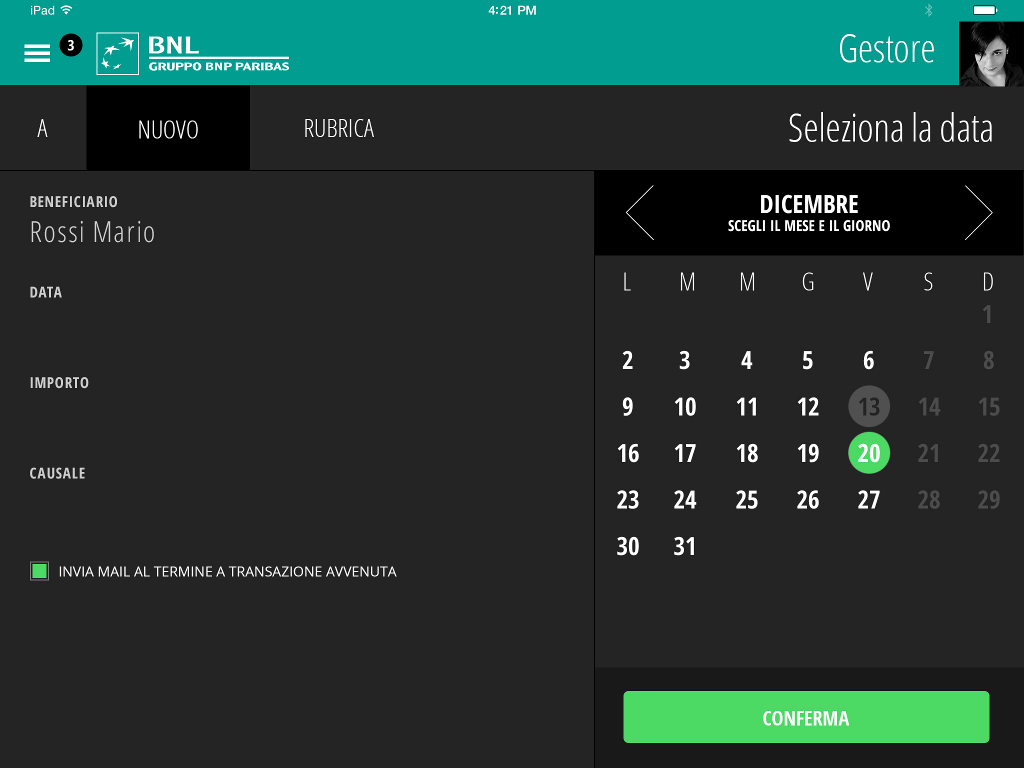
\includegraphics[scale=0.30]{ux/bonificonero.png}
\caption{Tema iniziale nero per la sezione bonifico}
\end{figure}

\begin{figure}[!htbp]
\centering
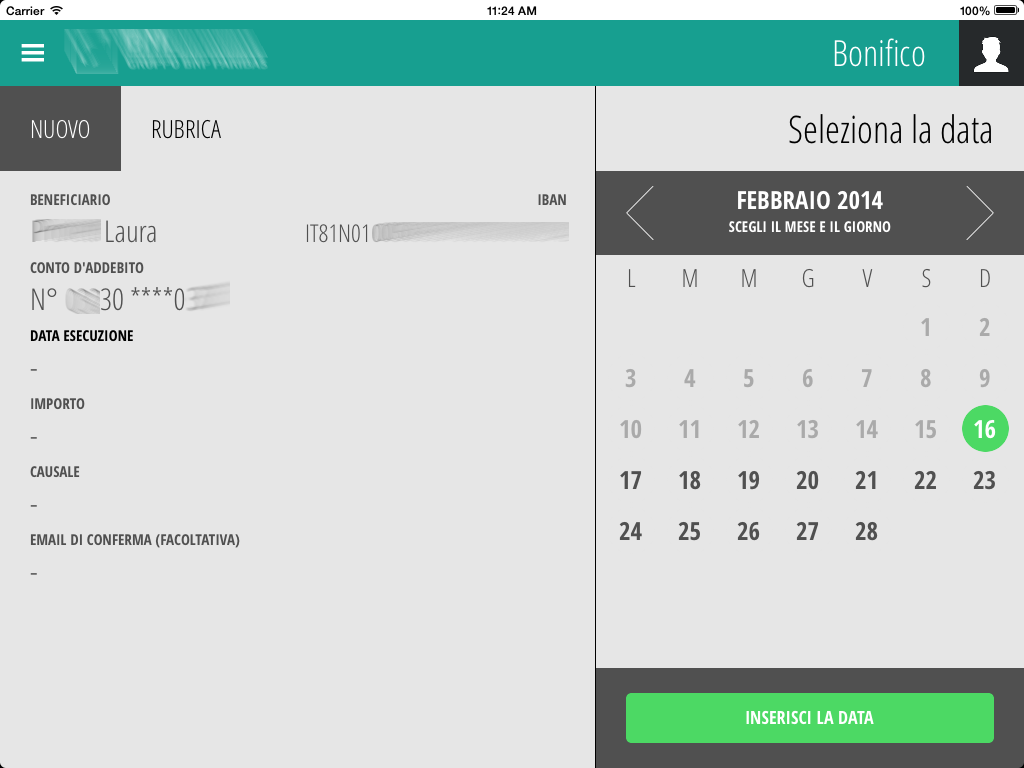
\includegraphics[scale=0.30]{ux/bonificogrigio.png}
\caption{Tema chiaro per il bonifico nella sua versione finale, si noti il pulsante \emph{conferma} in risalto rispetto altri elementi della GUI}
\end{figure}

\begin{figure}[!htbp]
\centering
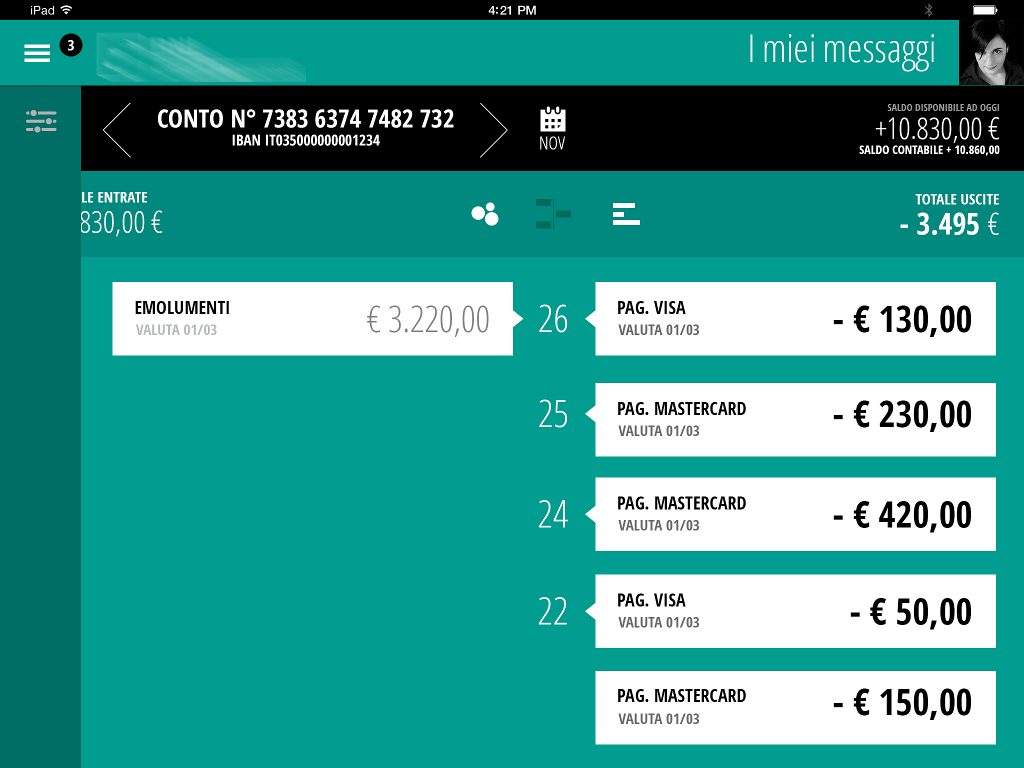
\includegraphics[scale=0.30]{ux/timeline3.png}
\caption{Tema verde per il background della timeline}
\end{figure}
\begin{figure}[!htbp]
\centering
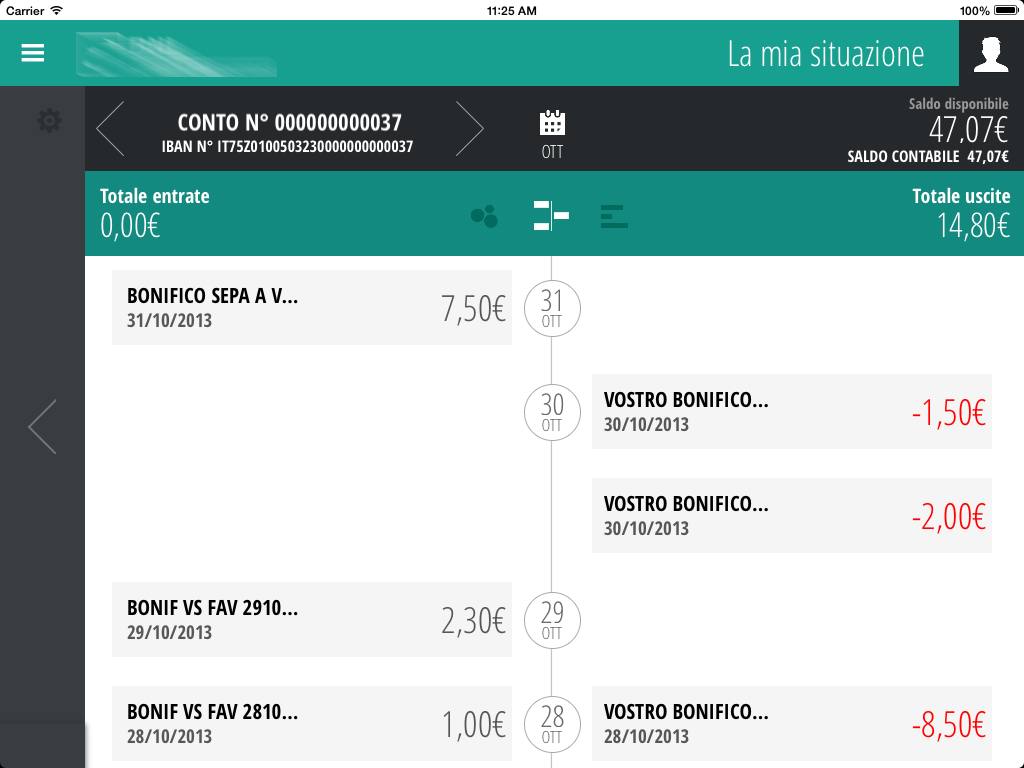
\includegraphics[scale=0.30]{ux/timelinebianca.png}
\caption{Tema chiaro per il background della timeline e utilizzo del colore rosso e grigio per dare risalto ai saldi negativi e positivi dei movimenti}
\end{figure}

\newpage
\subsubsection{Suggerimenti}

Dai test effettuati si è notata la necessita di aiutare l'utente attraverso suggerimenti (\emph{hint}) visivi posti in particolari punti delle interfacce. L'utilizzo moderato di suggerimenti ha aumentato e migliorato la \emph{discoverability}. 
\begin{figure}[!htbp]
\centering
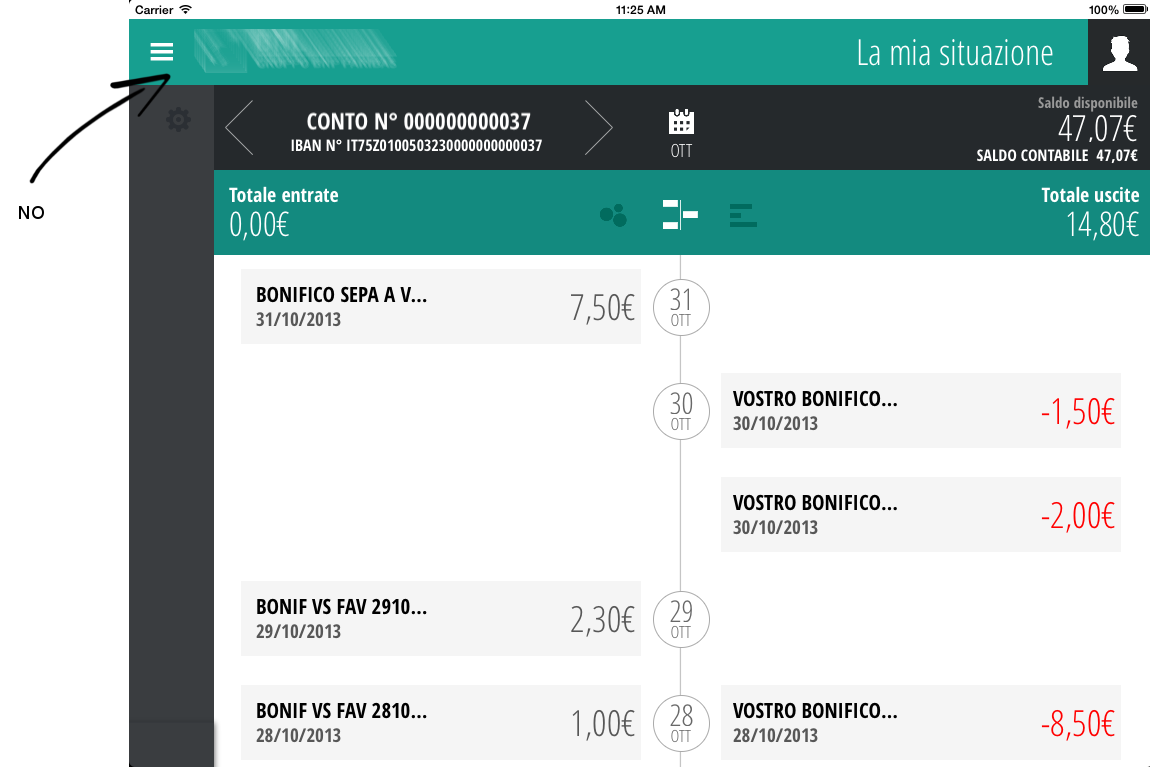
\includegraphics[scale=0.30]{ux/timelinenohint.png}
\caption{L'utente premeva il pulsante \emph{menu} per cercare di tornare alla schemata dei conti}
\end{figure}
\begin{figure}[!htbp]
\centering
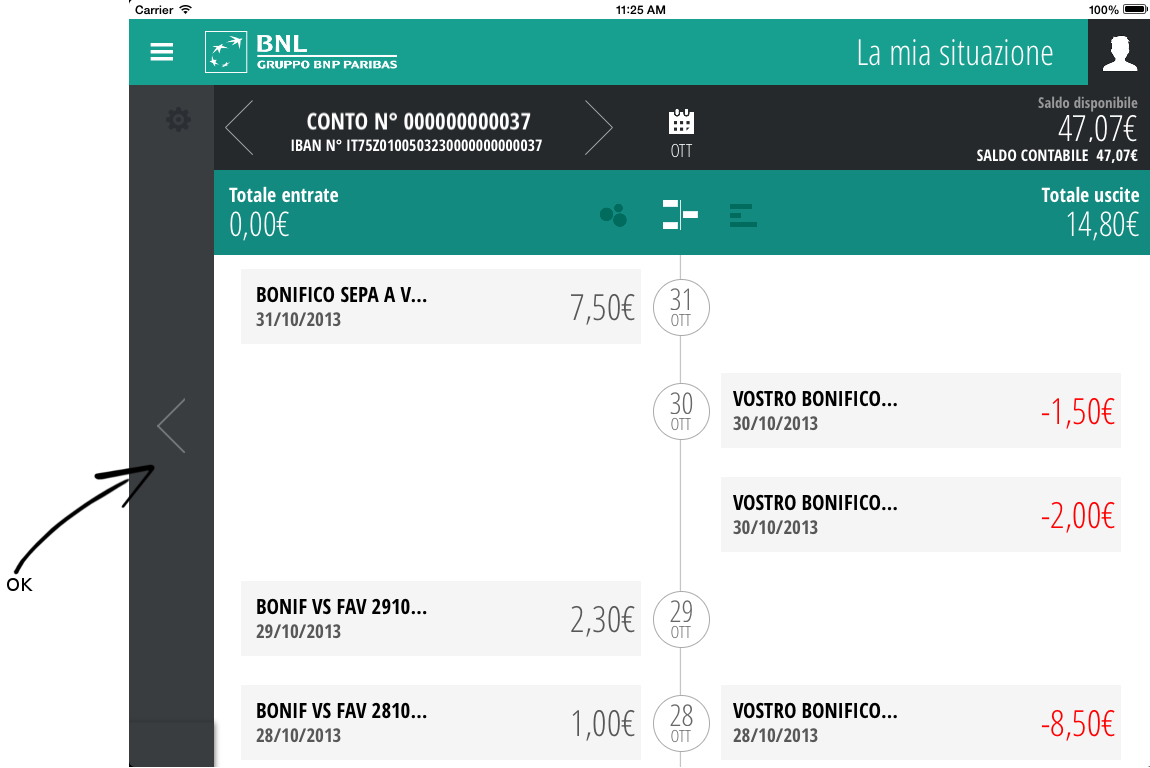
\includegraphics[scale=0.30]{ux/timelinehint.png}
\caption{Con una freccia che rappresentasse il significato di \emph{indietro} si è messo in risalto la relativa azione}
\end{figure}

\subsubsection{Feedback}
Per indicare che, in risposta ad una azione dell'utente, è avvenuto un evento nel sistema  si è scelto di utilizzare feedback visivi e diversificati in base al tipo di azione intrapresa. 
Di seguito sono riportati alcuni dei feedback utilizzati all'interno dell'applicazione:

\begin{itemize}
 \item componenti che indicano il caricamento durante task di lunga durata (esempio durante le chiamate http ai servizi, figura \ref{fig:loading})
 \item l'inserimento di animazioni per passare da un'interfacca ad un'altra dopo l'azione eseguita dall'utente (figura \ref{fig:animation})
 \item elementi grafici che cambiano il loro stati in risposta a eventi particolari (figura \ref{fig:copy})

\end{itemize}


\begin{figure}[htbp]
\centering
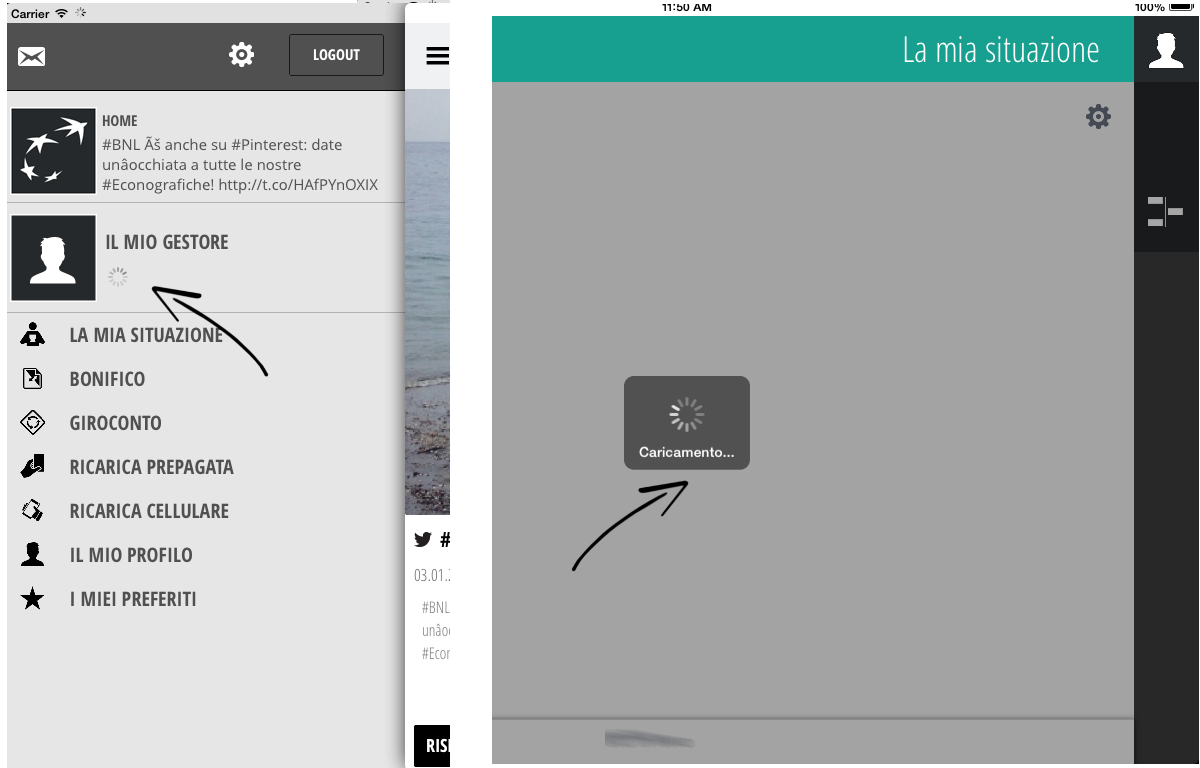
\includegraphics[scale=0.30]{ux/loading.png}
\caption{Esempi di loading view durante la chiamata ai servizi}
\label{fig:loading}
\end{figure}

\begin{figure}[htbp]
\centering
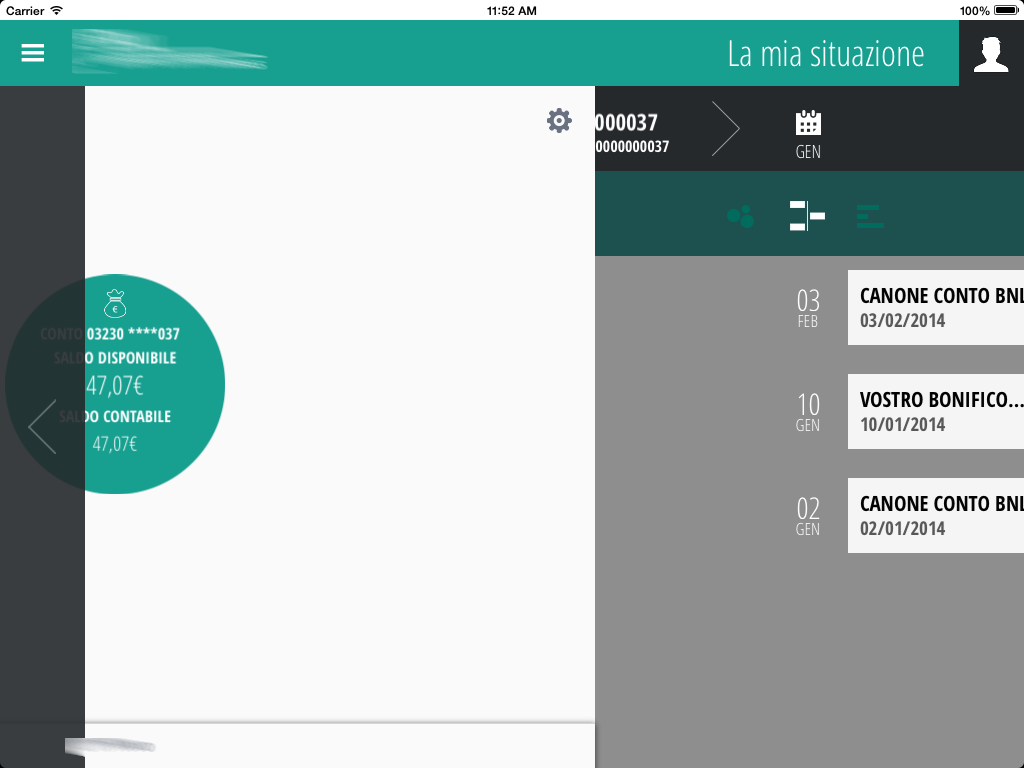
\includegraphics[scale=0.30]{ux/animazione.png}
\caption{Fotogramma preso durante un'animazione rappresentante il cambio di interfaccia e del relativo contesto (colori, immagini, contenuti)}
\label{fig:animation}
\end{figure}

\begin{figure}[htbp]
\centering
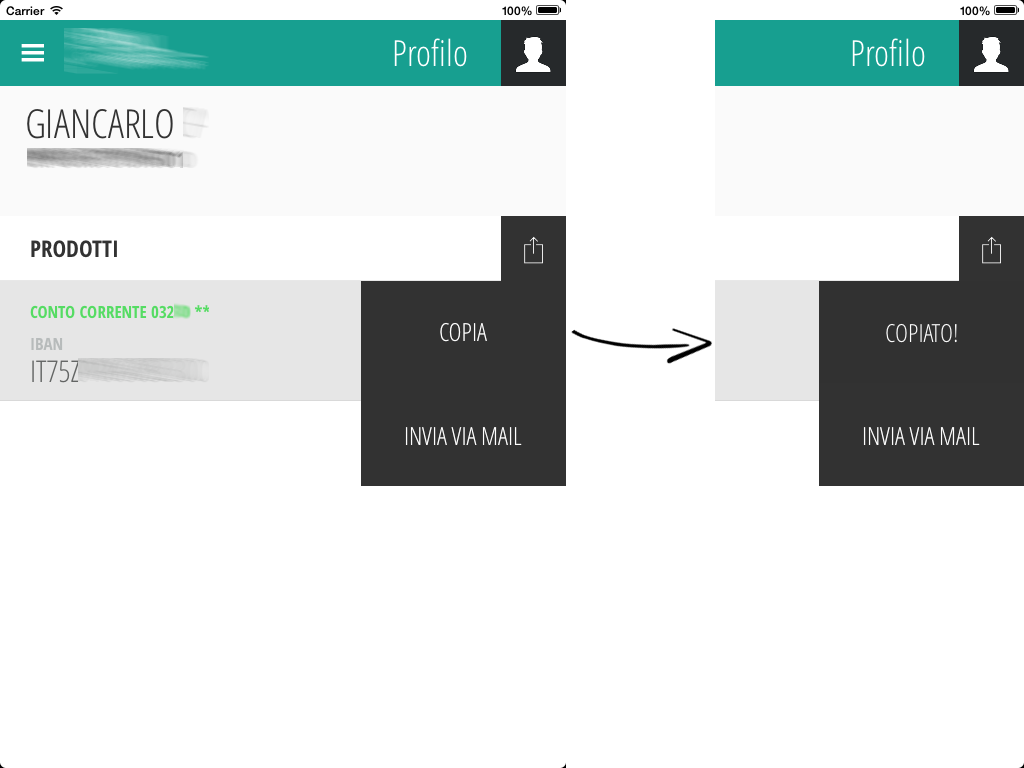
\includegraphics[scale=0.30]{ux/copia.png}
\caption{Dopo l'azione di copia il relativo pulsante cambia per qualche frazione di secondo il suo contenuto in \emph{copiato!}}
\label{fig:copy}
\end{figure}

\newpage
\subsubsection{Componenti personalizzati}
L'utilizzo di componenti grafici personalizzati ha permesso di ottenere interfacce grafiche più ricche di funzioni e al tempo stesso intuitive e facili da usare. La figura \ref{fig:selettore} rappresenta un componente grafico che ha la funzione di poter selezionare attraverso un tap sui pulsanti o attraverso la gesture swipe un elemento in una lista di oggetti (in questo caso di conti); tale componente è stato realizzato come libreria esterna, e quindi riusabile in diversi contesti della stessa applicazione.
\begin{figure}[htbp]
\centering
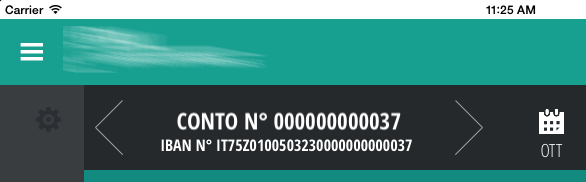
\includegraphics[scale=0.50]{ux/selettore.png}

\caption{Il componente custom \emph{selettore conti}}
\label{fig:selettore}
\end{figure}

\subsubsection{Prestazioni}
Per rendere più gradevole la user experience si è deciso di eseguire il \emph{caching}\footnote{Eseguire il salvataggio in ram o in memoria secondaria dei dati di frequente utilizzo, in modo tale da renderli disponibili per accessi futuri.} di alcuni dei dati scaricati dalla rete (come ad esempio la lista dei prodotti, o dati relativi al gestore, ecc\dots). Questa scelta ha quindi permesso di ridurre i tempi di accesso ad alcuni servizi migliorando le prestazioni del software in generale e l'interazione dell'utente con lo stesso.  